\section*{NP-Probleme}
\paragraph{SAT} Satisfiability ist eine beliebig lange Sequenz aus Wahrheitswerten, zu denen eine Lösung gesucht wird. 
\begin{align*}
    \varphi = (x_1, \dots , x_n)
\end{align*}
Ein Lösungszertifikat wird die Belegung der Variablen verlangt und überprüft, ob \(\varphi\)durch einsetzten der Werte wahr wird.
\paragraph{3SAT} Eine Variante von SAT ist 3SAT, welche nur Formeln in konjunktiver Normalsform vorkommen. Zudem hat jede Klausel genau 3 Therme.
\begin{align*}
    \varphi &= (x_1 \vee x_2 \vee x_3 ) \\
    &\wedge (\overline{x}_1 \vee \overline{x}_3 \vee \overline{x}_4) \\
    &\wedge ( x_1 \vee x_3 \vee x_5)
\end{align*}
\paragraph{k-Clique} Eine \(k\)-Clique ist eine Menge von \(k\) Ecken des Graphen, so dass im Graph jede Ecke der Teilmenge mit jeder anderen Ecke verbunden ist. Das Problem ist in \(O(n^k)\) lösbar. Als Lösungszertifikat verlangt man die Menge \(c = \{v_1, \dots , v_k \}\) der Vertizes der angeblichen Clique.
\paragraph{k-Vertex-Coloring} Die Vertizes eines Graphen können mit \(k\) Farben eingefärbt werden, wenn sich für jeden Vertex eine der \(k\) Farben wählen lässt, so dass nie zwei durch eine Kante verbundene Vertizes die gleiche Farbe bekommen. Das Problem ist eintscheidbar (man kann alle \(n^k\) möglichen Färbungen ausprobieren). Als Lösungszertifkat verlant man die Farbzuordnung \(c = (c_1, \dots, c_n)\) der Ecken \(1, \dots, n\) des Graphen. 
\paragraph{Hamiltonscher Pfad} Ein Hamiltonscher Pfad in einem gerichteten Graphen ist ein Pfad, der jeden Vertex des Graphen genau einmal besucht.
\paragraph{Binary Integer Programming} Für eine ganzzahlige Matrix \(C\) und einen ganzzahligen Vektor \(d\) soll ein binären Vektor \(x\) gefunden werden, sodass:
\begin{align*}
    Cx = d
\end{align*}
\paragraph{Vertex-Cover} Ein Graph \(G\) und eine Zahl \(k\). Gibt es eine Teilmenge von \(k\) Vertizes, sodass jede Kante von \(G\) ein Ende in dieser Teilmenge hat.\\
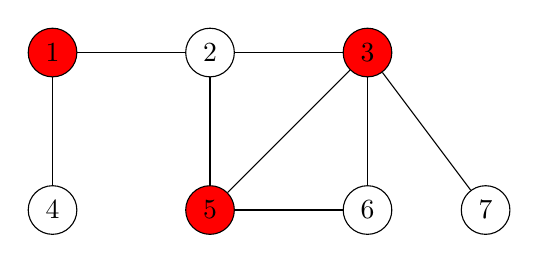
\begin{tikzpicture}
    \node[draw, circle, fill=red] (1) at (1,2) {1};
    \node[draw, circle] (4) at (1,0) {4};
    \node[draw, circle] (2) at (3,2) {2};
    \node[draw, circle, fill=red] (5) at (3,0) {5};
    \node[draw, circle, fill=red] (3) at (5,2) {3};
    \node[draw, circle] (6) at (5,0) {6};
    \node[draw, circle] (7) at (6.5,0) {7};
    \draw (1) -- (4);
    \draw (1) -- (2);
    \draw (2) -- (5);
    \draw (3) -- (5);
    \draw (2) -- (3);
    \draw (5) -- (6);
    \draw (3) -- (6);
    \draw (3) -- (7);
\end{tikzpicture}
\textbf{Telefonüberwachung:} Knoten sind die Anschlüsse, die Kanten verbinden die Anschlüsse welche tatsächlich miteinander telefonieren. Gesucht ist die Menge  aus\(k\) Knoten, sodass jedes mögliche Gespräch abgehört werden kann, also jede Kante in einem Knoten dieser Menge endet.
\paragraph{Feedback-Node-Set} Gegeben ein gerichteter Graph \(G\) und eine Zahl \(k\). Gibt es eine endliche Teilmenge von \(k\) Vertizes von \(G\) so, dass jeder Zyklus in \(G\) einen Vertex in der Teilmenge hat.\\
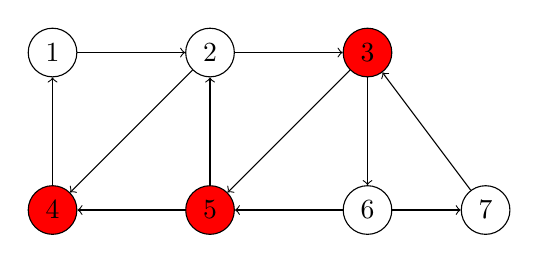
\begin{tikzpicture}
    \node[draw, circle] (1) at (1,2) {1};
    \node[draw, circle, fill=red] (4) at (1,0) {4};
    \node[draw, circle] (2) at (3,2) {2};
    \node[draw, circle, fill=red] (5) at (3,0) {5};
    \node[draw, circle, fill=red] (3) at (5,2) {3};
    \node[draw, circle] (6) at (5,0) {6};
    \node[draw, circle] (7) at (6.5,0) {7};
    \draw [<-] (1) -- (4);
    \draw [->] (1) -- (2);
    \draw [<-] (2) -- (5);
    \draw [->] (3) -- (5);
    \draw [->] (2) -- (3);
    \draw [<-] (5) -- (6);
    \draw [->] (3) -- (6);
    \draw [<-] (4) -- (5);
    \draw [->] (2) -- (4);
    \draw [<-] (3) -- (7);
    \draw [->] (6) -- (7);
\end{tikzpicture}\\
\textbf{Roboter:} Robter fahren Zyklen in einem gerichteten Graphen ab. Sie müssen durch regelmässig durch Prüfstellen fahren. Gesucht ist eine Menge von \(k\) Netzknoten sodass jeder Zyklus des Graphen durch eine dieser Prüfstellen verläuft.
\paragraph{Feedback-Arch-Set} Gegeben sei ein gerichteter Graph \(G\) und eine Zahl \(k\). Gibt es eine Teilmenge aus \(k\) Kanten, sodass jeder Zyklus in \(G\) eine Kante aus der Teilmenge enthält.\\
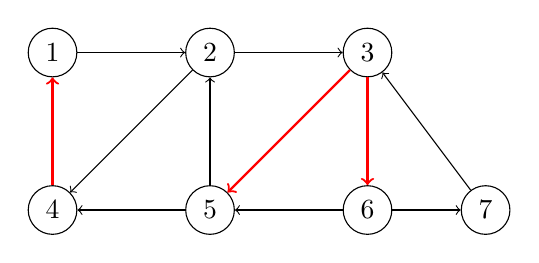
\begin{tikzpicture}
    \node[draw, circle] (1) at (1,2) {1};
    \node[draw, circle] (4) at (1,0) {4};
    \node[draw, circle] (2) at (3,2) {2};
    \node[draw, circle] (5) at (3,0) {5};
    \node[draw, circle] (3) at (5,2) {3};
    \node[draw, circle] (6) at (5,0) {6};
    \node[draw, circle] (7) at (6.5,0) {7};
    \draw [<-, color=red, thick] (1) -- (4);
    \draw [->] (1) -- (2);
    \draw [<-] (2) -- (5);
    \draw [->, color=red, thick] (3) -- (5);
    \draw [->] (2) -- (3);
    \draw [<-] (5) -- (6);
    \draw [->, color=red, thick] (3) -- (6);
    \draw [<-] (4) -- (5);
    \draw [->] (2) -- (4);
    \draw [<-] (3) -- (7);
    \draw [->] (6) -- (7);
\end{tikzpicture}\\
\textbf{Roboter:} Die Prüfstellen können die Roboter nun während er Fahrt prüfen. Gesucht ist eine Menge von \(k\) Kanten, sodass jeder Zyklus des Graphen über eine dieser Kanten führt.
\paragraph{Set-Covering} Gegeben eine endliche Familie endlicher Mengen \( (S_j)_{1\leq j\leq n} \) und eine Zahl \(k\). Gibt es eine Unterfamilie bestehend aus \(k\) Mengen, welche dieselbe Vereinigung haben.\\
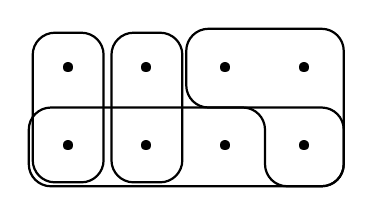
\begin{tikzpicture}[thick,rounded corners=8pt]
    \node at (1,1) {\textbullet};
    \node at (1,0) {\textbullet};
    \node at (2,1) {\textbullet};
    \node at (2,0) {\textbullet};
    \node at (3,1) {\textbullet};
    \node at (3,0) {\textbullet};
    \node at (4,0) {\textbullet};
    \node at (4,1) {\textbullet};
    \draw (0.5, -0.5) rectangle (4.5, 0.5);
    \draw (0.55, -0.45) rectangle (1.45, 1.45);
    \draw (1.55, -0.45) rectangle (2.45, 1.45);
    \draw (2.5, 1.5) -- (2.5, 0.5) -- (3.5, 0.5) -- (3.5, -0.5) -- (4.5, -0.5) -- (4.5, 1.5) -- cycle;
\end{tikzpicture}\\
\textbf{Steuererleichterungen} Jeder Wähler profitiert mindestens von einer Steuererleichterung. Es muss die kleinste Menge von Vereinigungen gefunden werden, sodass die gesamte Menge in der Vereinigung abgebildet ist. Die Steuervergünstigungen sind nummeriert \(1 \ldots n\). Sei \(S_j\) die Menge der Wähler, welche von Vergünstigung \(i\) profitieren. Es muss nun eine Teilmenge \(I= \{i_1, i_2, \ldots, i_k\} \) gefunden werden, dass die Vereinigungsmenge von Steuervergünstigungen der Wähler (\(S_j\)) und die Menge der Vergünstigung gleich sind. Also:
\begin{align*}
    \bigcup_{i=1}^n S_i = \bigcup_{i \in I} S_i
\end{align*}
\paragraph{Exact Cover} Gegeben eine Familie \( (S_j)_{1\leq j \leq n} \) von Teilmengen einer Menge \(U\). Gibt es eine Unterfamilie von Mengen, die disjunkt sind, aber die gleiche Vereinigung haben. Die Unterfamilie \( (S_{j_i})_{1\leq i \leq m} \) muss folgendes erfüllen:
\begin{align*}
    S_{j_i} \cap S_{j_k} &= \emptyset \\
    \bigcup_{j=1}^n S_j &= \bigcup_{i=1}^m S_{j_i}
\end{align*}\\
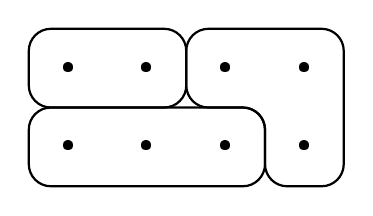
\begin{tikzpicture}[thick,rounded corners=8pt]
    \node at (1,1) {\textbullet};
    \node at (1,0) {\textbullet};
    \node at (2,1) {\textbullet};
    \node at (2,0) {\textbullet};
    \node at (3,1) {\textbullet};
    \node at (3,0) {\textbullet};
    \node at (4,0) {\textbullet};
    \node at (4,1) {\textbullet};
    \draw (0.5, -0.5) rectangle (3.5, 0.5);
    \draw (0.5, 0.5) rectangle (2.5, 1.5);
    \draw (2.5, 1.5) -- (2.5, 0.5) -- (3.5, 0.5) -- (3.5, -0.5) -- (4.5, -0.5) -- (4.5, 1.5) -- cycle;
\end{tikzpicture}\\
\textbf{Sträflingslager:} Die Menge aller Sträflinge ist \(U\). Die Projekte sind nummeriert: \(1 \ldots n\). Die Menge \( S_i \subset U \) besteht aus den Sträflingen, welche für das Projekt \( i\) ungeeignet sind. Weil jeder Sträfling für mindestens ein Projekt ungeeignet ist, ist:
\begin{align*}
    U = \bigcup_{i=1}^n S_i
\end{align*}
Gesucht ist die Teilmenge von Projekten \( I = \{ i_1, \ldots, i_m\} \subset \{1, \ldots, n \} \) sodass jeder Sträfling genau auf einem Projekt arbeitet, aber kein Sträfling mehr als einem Projekt zugeteilt ist:
\begin{align*}
    \bigcup_{j=1}^m S_{i_j} &= U \\
    S_{i_j} \cap S_{i_k} &= \emptyset \\
    \forall j \neq k
\end{align*}
\paragraph{Clique-Cover} Gegeben ist ein Graph und eine positive Zahl \(k\). Gibt es \(k\) Anzahl Cliquen, sodass jede Ecke in genau einer Clique ist.\\
\begin{comment}
\begin{tikzpicture}
    \node[draw, circle] (1) {1};
    \node[draw, circle] (7) [below left = of 1]{7};
    \node[draw, circle] (5) [below right = of 7] {5};
    \node[draw, circle] (4) [below right = of 1] {4};
    \draw [very thick, color=blue] (1) -- (7);
    \draw [very thick, color=blue] (1) -- (4);
    \draw [very thick, color=blue] (1) -- (5);
    \draw [very thick, color=blue] (4) -- (7);
    \draw [very thick, color=blue] (4) -- (5);
    \draw [very thick, color=blue] (5) -- (7);
    \node [draw, circle] (8) [below right = of 4] {8};
    \node [draw, circle] (2) [below right = of 8] {2};
    \node [draw, circle] (3) [below left = of 8] {3};
    \node [draw, circle] (6) [below right= of 3] {6};
    \draw [very thick, color=blue] (3) -- (2);
    \draw [very thick, color=blue] (3) -- (6);
    \draw [very thick, color=blue] (3) -- (8);
    \draw [very thick, color=blue] (2) -- (6);
    \draw [very thick, color=blue] (2) -- (8);
    \draw [very thick, color=blue] (6) -- (8);
\end{tikzpicture}\\
\end{comment}
\definecolor{qqqqff}{rgb}{0.,0.,1.}
\definecolor{cqcqcq}{rgb}{0.7529411764705882,0.7529411764705882,0.7529411764705882}
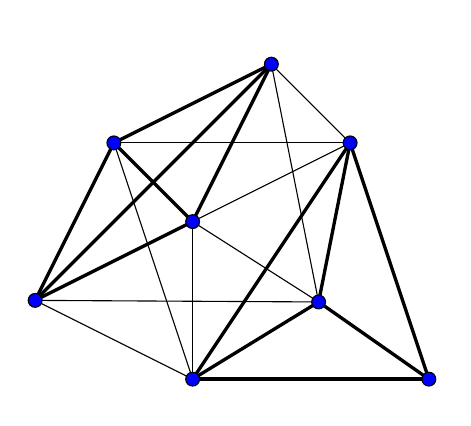
\begin{tikzpicture}[line cap=round, line join=round]
\draw [very thick] (1.,2.)-- (2.,4.);
\draw [very thick] (2.,4.)-- (4.,5.);
\draw [very thick] (4.,5.)-- (3.,3.);
\draw [very thick] (3.,3.)-- (1.,2.);
\draw [very thick] (2.,4.)-- (3.,3.);
\draw [very thick] (1.,2.)-- (4.,5.);
\draw [very thick] (3.,1.)-- (5.,4.);
\draw [very thick] (5.,4.)-- (4.6,1.98);
\draw [very thick] (4.6,1.98)-- (3.,1.);
\draw [very thick] (3.,1.)-- (6.,1.);
\draw [very thick] (6.,1.)-- (5.,4.);
\draw [very thick] (4.6,1.98)-- (6.,1.);
\draw (1.,2.)-- (3.,1.);
\draw (3.,1.)-- (2.,4.);
\draw (1.,2.)-- (4.6,1.98);
\draw (4.6,1.98)-- (4.,5.);
\draw (2.,4.)-- (5.,4.);
\draw (5.,4.)-- (4.,5.);
\draw (3.,3.)-- (4.6,1.98);
\draw (3.,1.)-- (3.,3.);
\draw (3.,3.)-- (5.,4.);
\begin{scriptsize}
\draw [fill=qqqqff] (1.,2.) circle (2.5pt);
\draw[color=qqqqff] (1.08,2.37) node {$$};
\draw [fill=qqqqff] (2.,4.) circle (2.5pt);
\draw[color=qqqqff] (2.08,4.37) node {$$};
\draw [fill=qqqqff] (4.,5.) circle (2.5pt);
\draw[color=qqqqff] (4.08,5.37) node {$$};
\draw [fill=qqqqff] (3.,3.) circle (2.5pt);
\draw[color=qqqqff] (3.08,3.37) node {$$};
\draw [fill=qqqqff] (3.,1.) circle (2.5pt);
\draw[color=qqqqff] (3.08,1.37) node {$$};
\draw [fill=qqqqff] (4.6,1.98) circle (2.5pt);
\draw[color=qqqqff] (4.68,2.35) node {$$};
\draw [fill=qqqqff] (5.,4.) circle (2.5pt);
\draw[color=qqqqff] (5.08,4.37) node {$$};
\draw [fill=qqqqff] (6.,1.) circle (2.5pt);
\draw[color=qqqqff] (6.08,1.37) node {$$};
\draw[color=black] (1.78,3.03) node {$$};
\draw[color=black] (3.14,4.39) node {$$};
\draw[color=black] (3.2,4.33) node {$$};
\draw[color=black] (1.84,2.97) node {$$};
\draw[color=black] (2.26,3.45) node {$$};
\draw[color=black] (2.72,3.45) node {$$};
\draw[color=black] (4.26,2.51) node {$$};
\draw[color=black] (4.48,3.23) node {$$};
\draw[color=black] (3.62,1.95) node {$$};
\draw[color=black] (4.5,0.85) node {$$};
\draw[color=black] (5.8,2.79) node {$$};
\draw[color=black] (5.1,1.41) node {$$};
\draw[color=black] (1.84,1.39) node {$$};
\draw[color=black] (2.8,2.79) node {$$};
\draw[color=black] (2.78,1.85) node {$$};
\draw[color=black] (4.6,3.73) node {$$};
\draw[color=black] (3.5,3.85) node {$$};
\draw[color=black] (4.72,4.91) node {$$};
\draw[color=black] (3.62,2.41) node {$$};
\draw[color=black] (3.32,2.17) node {$$};
\draw[color=black] (4.14,3.39) node {$$};
\end{scriptsize}
\end{tikzpicture}
\textbf{Gruppenarbeit:} Für eine Gruppenarbeit sollen \(k\) Gruppen gebildet werden. Die Leute einer Gruppe sollen sich bereits gegenseitig kennen und alle Leute sollen beschäftigt sein. \\
\textbf{Weak-Clique-Cover:} Hier wird nicht verlangt, dass die Cliquen disjunkt sind.
\paragraph{3D-Matching} Sei \(T\) eine endliche Menge und \(U\) eine Menge von Tripeln aus \(T: U \subset T \times T \times T\). Gibt es eine Teilmenge \(W \subset U\), sodass \(\vert W \vert = \vert T \vert\) und keine zwei Elemente von \(W\) stimmen in irgendeiner Koordinate überein.\\
\textbf{Marsbewohner:} Auf dem Mars lebt eine Spezies mit drei Geschlechter. Von allen Geschlechtern gibt es genau \(n\) Personen. Es muss nun eine Liste aus Tripeln erstellt werden, um alle diese Personen in einer "{}Dreier“{}-Ehe verheiraten zu können.\\
\textbf{Zwangsheirat:} Es gibt \(n\) unverheiratete Frauen, Männer und Wohnungen. Es ist eine Liste mit einer Menge von Tripeln erstellt worden \((x,y,z)\), wobei die Zahlen \(x\), \(y\) und \(z\) aus der Menge \(T = [n] = \{1, \ldots, n\} \) stammen. Aus dieser Teilmenge \(U \subset T \times T \times T \) soll jetzt eine Teilmenge \(W \subset U\) von genau \(n\) Tripeln ausgewählt werden, sodass jedes Mann, jede Frau und jede Wohnung genau in einem Tripel vorkommt.
\paragraph{Hitting-Set} Gegeben ist eine Menge von Teilmengen \(S_i \subset S\). Gibt es eine Menge \(H\) die jede Menge genau in einem Punkt trifft:
\begin{align*}
    \vert H \cap S_i \vert = 1\forall i
\end{align*}
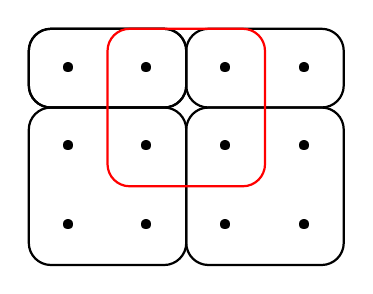
\begin{tikzpicture}[thick,rounded corners=8pt]
    \node at (1,1) {\textbullet};
    \node at (1,0) {\textbullet};
    \node at (2,1) {\textbullet};
    \node at (2,0) {\textbullet};
    \node at (3,1) {\textbullet};
    \node at (3,0) {\textbullet};
    \node at (4,0) {\textbullet};
    \node at (4,1) {\textbullet};
    \node at (1,2) {\textbullet};
    \node at (2,2) {\textbullet};
    \node at (3,2) {\textbullet};
    \node at (4,2) {\textbullet};
    \draw (0.5, -0.5) rectangle (2.5, 1.5);
    \draw (2.5, -0.5) rectangle (4.5, 1.5);
    \draw (0.5, 2.5) rectangle (2.5, 1.5);
    \draw (2.5, 1.5) rectangle (4.5, 2.5);
    \draw (0.5, 1.5) rectangle (2.5, 2.5);
    \draw[color=red] (1.5,0.5) rectangle (3.5,2.5);
% Diese Menge würde das HS verletzen
%    \draw (1.55,-0.45) rectangle (3.45,1.45);
\end{tikzpicture}\\
\textbf{Fachgebiet:}Sei \(S_i\) eine Menge von Wissenschaftlern, die zum Thema \(i\) Stellung beziehen können. Gesucht ist eine Auswahl \(H\) von Wissenschaftlern, sodass jeder Wissenschaftler genau ein Fachgebiet hat, für das er Stellung nehmen kann, also:
\begin{align*}
    \vert H \cap S_i \vert = 1
\end{align*}
\paragraph{Steiner-Tree} Gegeben ist ein Graph, eine Teilmenge \(R\) von Vertizes und eine Gewichtsfunktion \(w: E \mapsto \mathbb{Z}\) und eine positive Zahl \(k\). Gibt es einen Baum mit Gewicht \(\leq k\), dessen Knoten in \(R\) enhtalten sind. Das Gewicht des Baumes ist die Summer der Gewichte \(w(\{u,v\})\) über alle Kanten \(\{u,v\}\) im Baum.\\
\begin{tikzpicture}
        \node [draw, circle, fill=red] (A) at (1,1) {A};
        \node [draw, circle, right = 3cm of A] (B) {B};
        \node [draw, circle, fill=green, below = 2 cm of A] (C) {C};
        \node [draw, circle, fill=red, right = 3cm of C] (D) {D};
        \draw [ultra thick] (A) -- node[left]{2} (C);
        \draw [ultra thick] (C) -- node[below]{10} (D);
        \draw (A) -- node[above]{5} (B);
        \draw (B) -- node[right]{20} (D);
\end{tikzpicture}\\
\textbf{Geldtransport:} Bankgesellschaft möchte Filialen mit Geld versorgen. Geldtransporte sollen auch zwischen Filialen möglich sein. Vom Hauptsitz werden Beträge für mehrere Filialen verladen. Die Filialen nehmen die Lieferung ausseinander und laden sie auf neue Transporte. Die Frage ist, ob es möglich ist, mit dieser Methode die Kosten unter den Betrag \(k\) zu senken.
\paragraph{Sequencing} Gegeben sei ein Vektor \((t_1, \dots, t_p) \in \mathbb{Z}^p\) von Laufzeiten von Jobs, ein Deadline Vektor \((d_1, \dots, d_p) \in \mathbb{Z}^p \), einem Strafenvektor \((s_1, \dots, s_p) \in \mathbb{Z}^p\) und eine positive Ganzzahl \(k\). Gibt es eine Permutation \(\pi\) der Zahlen \(1, \dots, p\) sodass die Gesamtstrafe für verspätete Ausführung bei der Ausführung der Jobs in der Reihenfolge \(\pi(1), \dots, \pi(p)\) nicht grösser als \(k\) ist.\\
\begin{tabular}{l|lll}
\hline
Job & Dauer & Deadline & Strafe \\ \hline
T1  & 4     & 5        & 30     \\
T2  & 1     & 3        & 25     \\
T3  & 2     & 2        & 20     \\ \hline
\end{tabular}\\
\textbf{Züge:} Die Durchfahrzeit des Zuges \(i\) durch die Strecke ist \(t_i\). Wenn der Zug später als \(d_i\) ankommt ist die Strafe \(s_i\) fällig. Wenn die Züge in der durch die Permutation \(\pi\) permutierten Reihenfolge \(\pi(1), \pi(2), \ldots, \pi(n)\) abgefertigt, beträgt die für Zug \(j\) anfallende Strafe: \(\vartheta(t_{\pi(1)} + \ldots + t_{\pi(j)})_{S_\pi(j)}\). Die Gesamtstrafe ist daher:
\begin{align*}
    \sum_{j=1}^n \vartheta(t_{\pi(1)} + \ldots + t_{\pi(j)})_{S_\pi(j)}
\end{align*}
\paragraph{Subset-Sum} Gegeben ist eine Menge \(S\) von ganzen Zahlen. Kann darin eine Teilmenge gefunden werden, die als Summe einen bestimmten Wert \(t\) hat.
\textbf{Jahresbudget:} Die Vorschläge des Teams, das Jahresbudget aufzubrauchen, bildet die Menge \(\{b_1, \ldots, b_n\}\) von Beträgen \(b_i\). Daraus soll eine Teilmenge \(I=\{i_1, \ldots, i_m\}\) gebildet werden, sodass der Restbetrag \(r\) aufgebraucht wird.
\begin{align*}
    \sum_{k=1}^m b_{i_k} = r
\end{align*}
\paragraph{Partition} Gegeben ist eine Folge von \(s\) ganzen Zahlen: \(c_1, \ldots c_s\). Kann man die Indizes \(1, \ldots, s\) in zwei Teilmengen \(I\) und \(\overline{I}\) teilen, sodass die Summer der zugehörigen Zahlen identisch ist.
\begin{align*}
    \sum_{i\in I} c_i = \sum_{i \notin I} c_i
\end{align*}
\textbf{Köngiserbe:} Zwei Söhne eines verstorbenen Königs sollten genau denselben Betrag erben. Der Wert der Immobilie \(i\) ist mit \(c_i\) beziffert. Die Aufgabe besteht nun darin, eine Aufteilung zu der Menge \(A\) aller Immobilien zu finden, damit in die Summe der Mengen \(I\) und \(A\setminus I\) genau diesselbe ist.
\begin{align*}
        \sum_{i\in I} c_i = \sum_{i \in A\setminus I} c_i    
\end{align*}
\paragraph{Max-Cut} Gegeben ist ein Graph mit einer Gewichtsfunktion \(w: E \mapsto \mathbb{Z}\) und eine Ganzzahl \(W\). Gibt es eine Teilmenge \(S\) der Vertizes, so dass das Gesamtgewicht der Kanten die \(S\) mit seinem Komplement verbinden, mindestens so gross ist wie \(W\):
\begin{align*}
    \sum_{\{u,v\}\in E \wedge u \in S \wedge v \notin S} w(\{u,v\}) \geq W
\end{align*}
\begin{tikzpicture}
    \draw [very thick](-1.5,-0.5) -- (3.5,-2.5);
    \node [draw, circle] (a) {a};
    \node [draw, circle, below = 2cm of a] (b) {b};
    \node [draw, circle, below left= 1.25cm of a] (s) {s};
    \node [draw, circle, right= 1.5cm of a] (c) {c};
    \node [draw, circle, right= 1.5cm of b] (d) {d};
    \node [draw, circle, below right= 1.25cm of c] (t) {t};
    \draw [->] (s) -- node[above]{3} (a);
    \draw [->] (s) -- node[below]{2} (b);
    \draw [->] (a) -- node[left]{1} (b);
    \draw [->] (a) -- node[above]{3} (c);
    \draw [->] (a) -- node[above]{4} (d);
    \draw [->] (b) -- node[above]{2} (d);
    \draw [->] (c) -- node[above]{2} (t);
    \draw [->] (d) -- node[above]{3} (t);
\end{tikzpicture}
\textbf{Grenzhandel:} Die Produktionsstationen bilden einen Graphen, dessen Kanten anzeigen, ob zwischen den beiden Stationen ein Transport notwendig ist. Jede Kante ist der mögliche Gewinn zugeordnet, der winkt, wenn der Transport grenzquerend durchgeführt werden kann. Gesucht wird eine Aufteilung der Produktionsstationen auf die beiden Landesteile so dass der Gewinn aus Subventionen die Ziele \(W\) des Managements übersteigen.
\paragraph{Set-Packing} Gegeben eine Familie \( (S_i)_{i \in I} \) von Mengen und eine positive Ganzzahl \(k\). Gibt es eine \(k\)-elementige Teilfamilie \( (S_i)_{i \in J} \) mit \( J \subset I \), dass die Mengen der Teilfamilie paarweise disjunkt sind:
\begin{align*}
    \vert J \vert &= k \\
    S_i \cap S_j &= \emptyset \\
    \forall i,j &\in J \text{ mit } i \neq j
\end{align*}
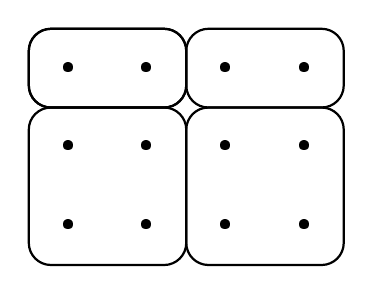
\begin{tikzpicture}[thick,rounded corners=8pt]
    \node at (1,1) {\textbullet};
    \node at (1,0) {\textbullet};
    \node at (2,1) {\textbullet};
    \node at (2,0) {\textbullet};
    \node at (3,1) {\textbullet};
    \node at (3,0) {\textbullet};
    \node at (4,0) {\textbullet};
    \node at (4,1) {\textbullet};
    \node at (1,2) {\textbullet};
    \node at (2,2) {\textbullet};
    \node at (3,2) {\textbullet};
    \node at (4,2) {\textbullet};
    \draw (0.5, -0.5) rectangle (2.5, 1.5);
    \draw (2.5, -0.5) rectangle (4.5, 1.5);
    \draw (0.5, 2.5) rectangle (2.5, 1.5);
    \draw (2.5, 1.5) rectangle (4.5, 2.5);
    \draw (0.5, 1.5) rectangle (2.5, 2.5);
\end{tikzpicture}\\
\textbf{Medizinische Studie:} F"ur eine medizinische Studie ist eine grosse Zahl von Probanden rekrutiert worden. Sie sind bereits auf Allergien getestet worden, man weiss also von jedem Probanden, auf welche Allergene er allergisch reagiert. Die Untersuchung soll sich auf eine Teilmenge von $k=17$ oder noch mehr ausgew"ahlten Allergenen beschr"anken, die so beschaffen ist, dass kein Proband auf mehr als  eines der ausgew"ahlten Allergene reagiert.
\paragraph{Damen-Problem}
Das Acht-Damen-Problem ist die Schach-Aufgabe, acht Damen so auf einem
Schachbrett aufzustellen, dass sie sich nicht gegenseitig schlagen k"onnen.
Eine Dame kann eine andere Figur schlagen, die sich in der gleichen Zeile,
Spalte oder Diagonale befindet.
Offenbar ist acht die maximale Anzahl von Damen, die man auf diese Art auf
einem Schachbrett platzieren kann.

Betrachten Sie jetzt das allgemeinere Problem
\[
\textsl{DAMEN}
=
\left\{\; n
\;\left|\;
\begin{minipage}{0.5\hsize}
Es gibt eine Platzierung von $n$ Damen auf einem $n\times n$-Schachbrett,
die sich nicht gegenseitig schlagen k"onnen
\end{minipage}\right.\right\}.
\]
\begin{itemize}
\item
Konstruieren Sie eine Reduktion von \textsl{DAMEN} auf \textsl{SAT}.
\item
Bestimmen Sie den Rechenaufwand Ihrer Konstruktion in Abh"angigkeit von $n$.
\end{itemize}

\begin{itemize}
\item
Wir m"ussen f"ur jede Zahl $n$ eine Formel $\varphi_n$ in den Variablen
$x_{ij}$ mit $1\le i,j\le n$ konstruieren, die genau dann erf"ullbar ist,
wenn sich $n$ Damen auf dem Feld platzieren lassen, die sich nicht schlagen
lassen.

Diese Formel muss ausdr"ucken, dass in der gleichen Zeile, Spalte und
Diagonalen keine weitere Dame steht.
Wenn auf dem Feld $(i,j)$ eine Dame steht, dann wird dies gem"ass Hinweis
dadurch ausgedr"uckt, dass $x_{ij}$ wahr ist.
Wir m"ussen daher eine Formel bauen, die sicherstellt, dass in diesem Fall
alle $x_{kl}$ falsch sind, die zur gleichen Zeile, Spalte oder Diagonalen
geh"oren.

Wir schreiben $\oplus$ f"ur die XOR-Verkn"upfung.
Die Bedingung, dass keine weiteren Damen in der gleichen Zeile stehen,
kann man durch die Formel
\begin{align}
\varphi_{ij,\text{Zeile}}
&=
x_{ij}\oplus \\
&(x_{i1}\vee \dots \vee \hat x_{ij}\vee\dots\vee x_{in})
\label{70000036:oder}
\\
&=
x_{ij}\oplus\biggl(\bigvee_{k\ne j} x_{ik}\biggr)
\notag
\intertext{ausdr"ucken. Dabei bedeutet $\hat x_{ij}$, dass die Variable
$x_{ij}$ in der Klammer auf der rechten Seite weggelassen werden soll.
Analog kann man auch die Bedingungen f"ur die Spalten und die Diagonalen
ausdr"ucken:}
\varphi_{ij,\text{Spalte}}
&=
x_{ij}\oplus\\
&(x_{1j}\vee\dots\vee\hat x_{ij}\vee\dots\vee x_{nj})
\notag
\\
&=
x_{ij}\oplus\biggl(\bigvee_{l\ne i} x_{lj}\biggr),
\notag
\\
\varphi_{ij,\text{Diagonalen}}
&=
x_{ij}\oplus\biggl(\bigvee_{\text{$k,l$ diagonal von $i,j$}}x_{kl}\biggr).
\notag
\end{align}
Die Variablen $x$ repr"asentieren genau dann eine akzeptable Platzierung
wenn f"ur jedes Paar $(i,j)$ alle drei soeben entwickelten Formeln wahr werden:
\[
\varphi_{ij}
=
\varphi_{ij,\text{Zeile}}
\wedge
\varphi_{ij,\text{Spalte}}
\wedge
\varphi_{ij,\text{Diagonalen}}.
\]
Die gesuchte Formel ist daher
\[
\varphi = \bigwedge_{i,j=1}^n \varphi_{ij}.
\]
\item
F"ur den Aufbau dieser Formel braucht f"ur jedes Paar $(i,j)$ den gleichen
Aufwand $O(n)$.
Es gibt $n^ 2$ solche Paare, der gesamte Aufwand ist daher $O(n^3)$.
\end{itemize}



